\subsection{Referencia}

La empresa requirió que se utilizara un brazo robótico en 3D diseñado por la propia empresa, e incluido en el software SettDev, para ser empleado como referencia del movimiento realizado por la ortesis. La Figura \ref{fig:referencia} muestra el brazo en 3D diseñado por la propia empresa. Este modelo tiene 3 grados de libertad, y un grado de libertad adicional para el efector final (Muñeca). Puede notarse que en la parte superior hay controles deslizantes. La empresa requirió que estos controles se movieran de acuerdo con los ángulos obtenidos directamente de los sensores. Se asignó un sensor y eje fijos para un grado de libertad específico; el eje X y eje Z del sensor colocado en el codo controlan el movimiento de la base y el antebrazo, respectivamente, mientras que el eje Z del sensor colocado en el extremo de la ortesis controla el movimiento del antebrazo. El eje Y del sensor colocado en la mano controla el movimiento de la muñeca.

\begin{figure}[htb]
	\centering
	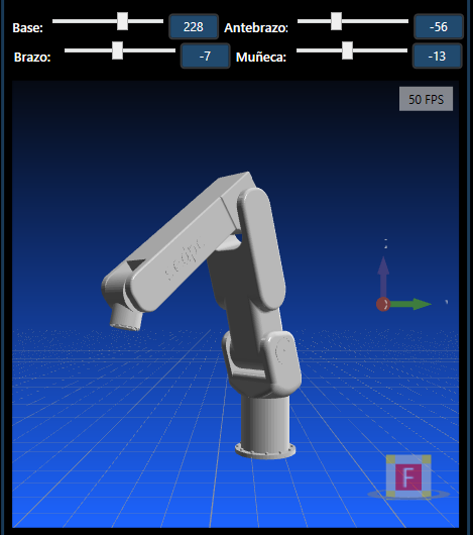
\includegraphics[scale=0.6]{referencia.png}
	\caption{Brazo en 3D utilizado como referencia en el software SettDev}
	\label{fig:referencia}
\end{figure}